\subsection{Reproduction du XOR}

\begin{frame}{L'opérateur XOR}
	\begin{block}{Le XOR nécessite un réseau}
		Le XOR, \og $ou\ exclusif$ \fg, est un opérateur non linéairement séparable. \\
	\end{block}
    \begin{columns}
        \begin{column}{0.6\textwidth}
            \begin{figure}
                \centering
                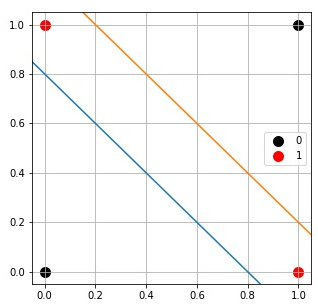
\includegraphics[width=150px]{2-XOR.jpg}
                \caption{Schéma de l'opérateur XOR}
            \end{figure}
        \end{column}
        \begin{column}[]{0.3\textwidth}
            \begin{center}
                \begin{tabular}{|c c | c|}
                    \hline
                    A & B & A xor B \\ \hline
                    0 & 0 & 0 \\
                    0 & 1 & 1 \\
                    1 & 0 & 1 \\
                    1 & 1 & 0 \\
                    \hline
                \end{tabular}
                \end{center}
        \end{column}
    \end{columns}
\end{frame}



\begin{frame}{Le réseau de neurone reproduisant l'opérateur XOR}
	\begin{figure}
		\centering
		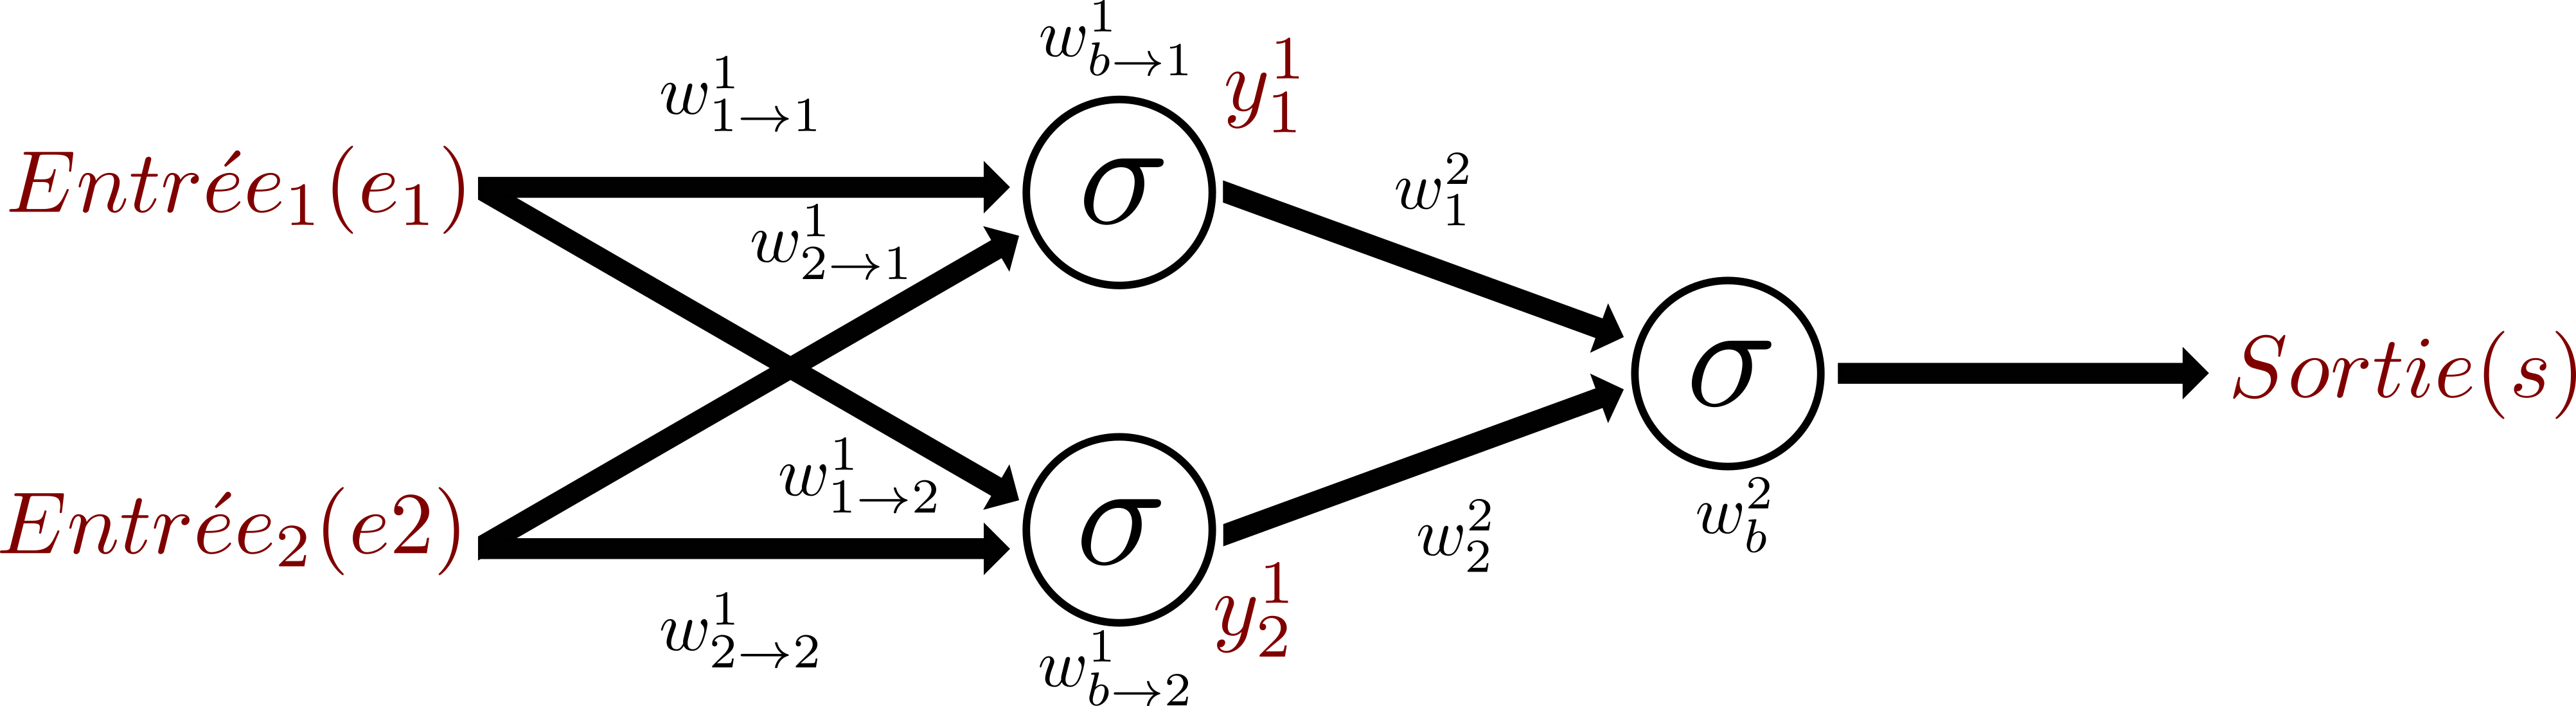
\includegraphics[width=\textwidth]{3-Model.png}
		\caption{Schéma du réseau de neurone reproduisant le XOR}
	\end{figure}
\end{frame}

\begin{frame}{L'apprentissage de la reproduction du XOR}
	\begin{figure}
		\centering
		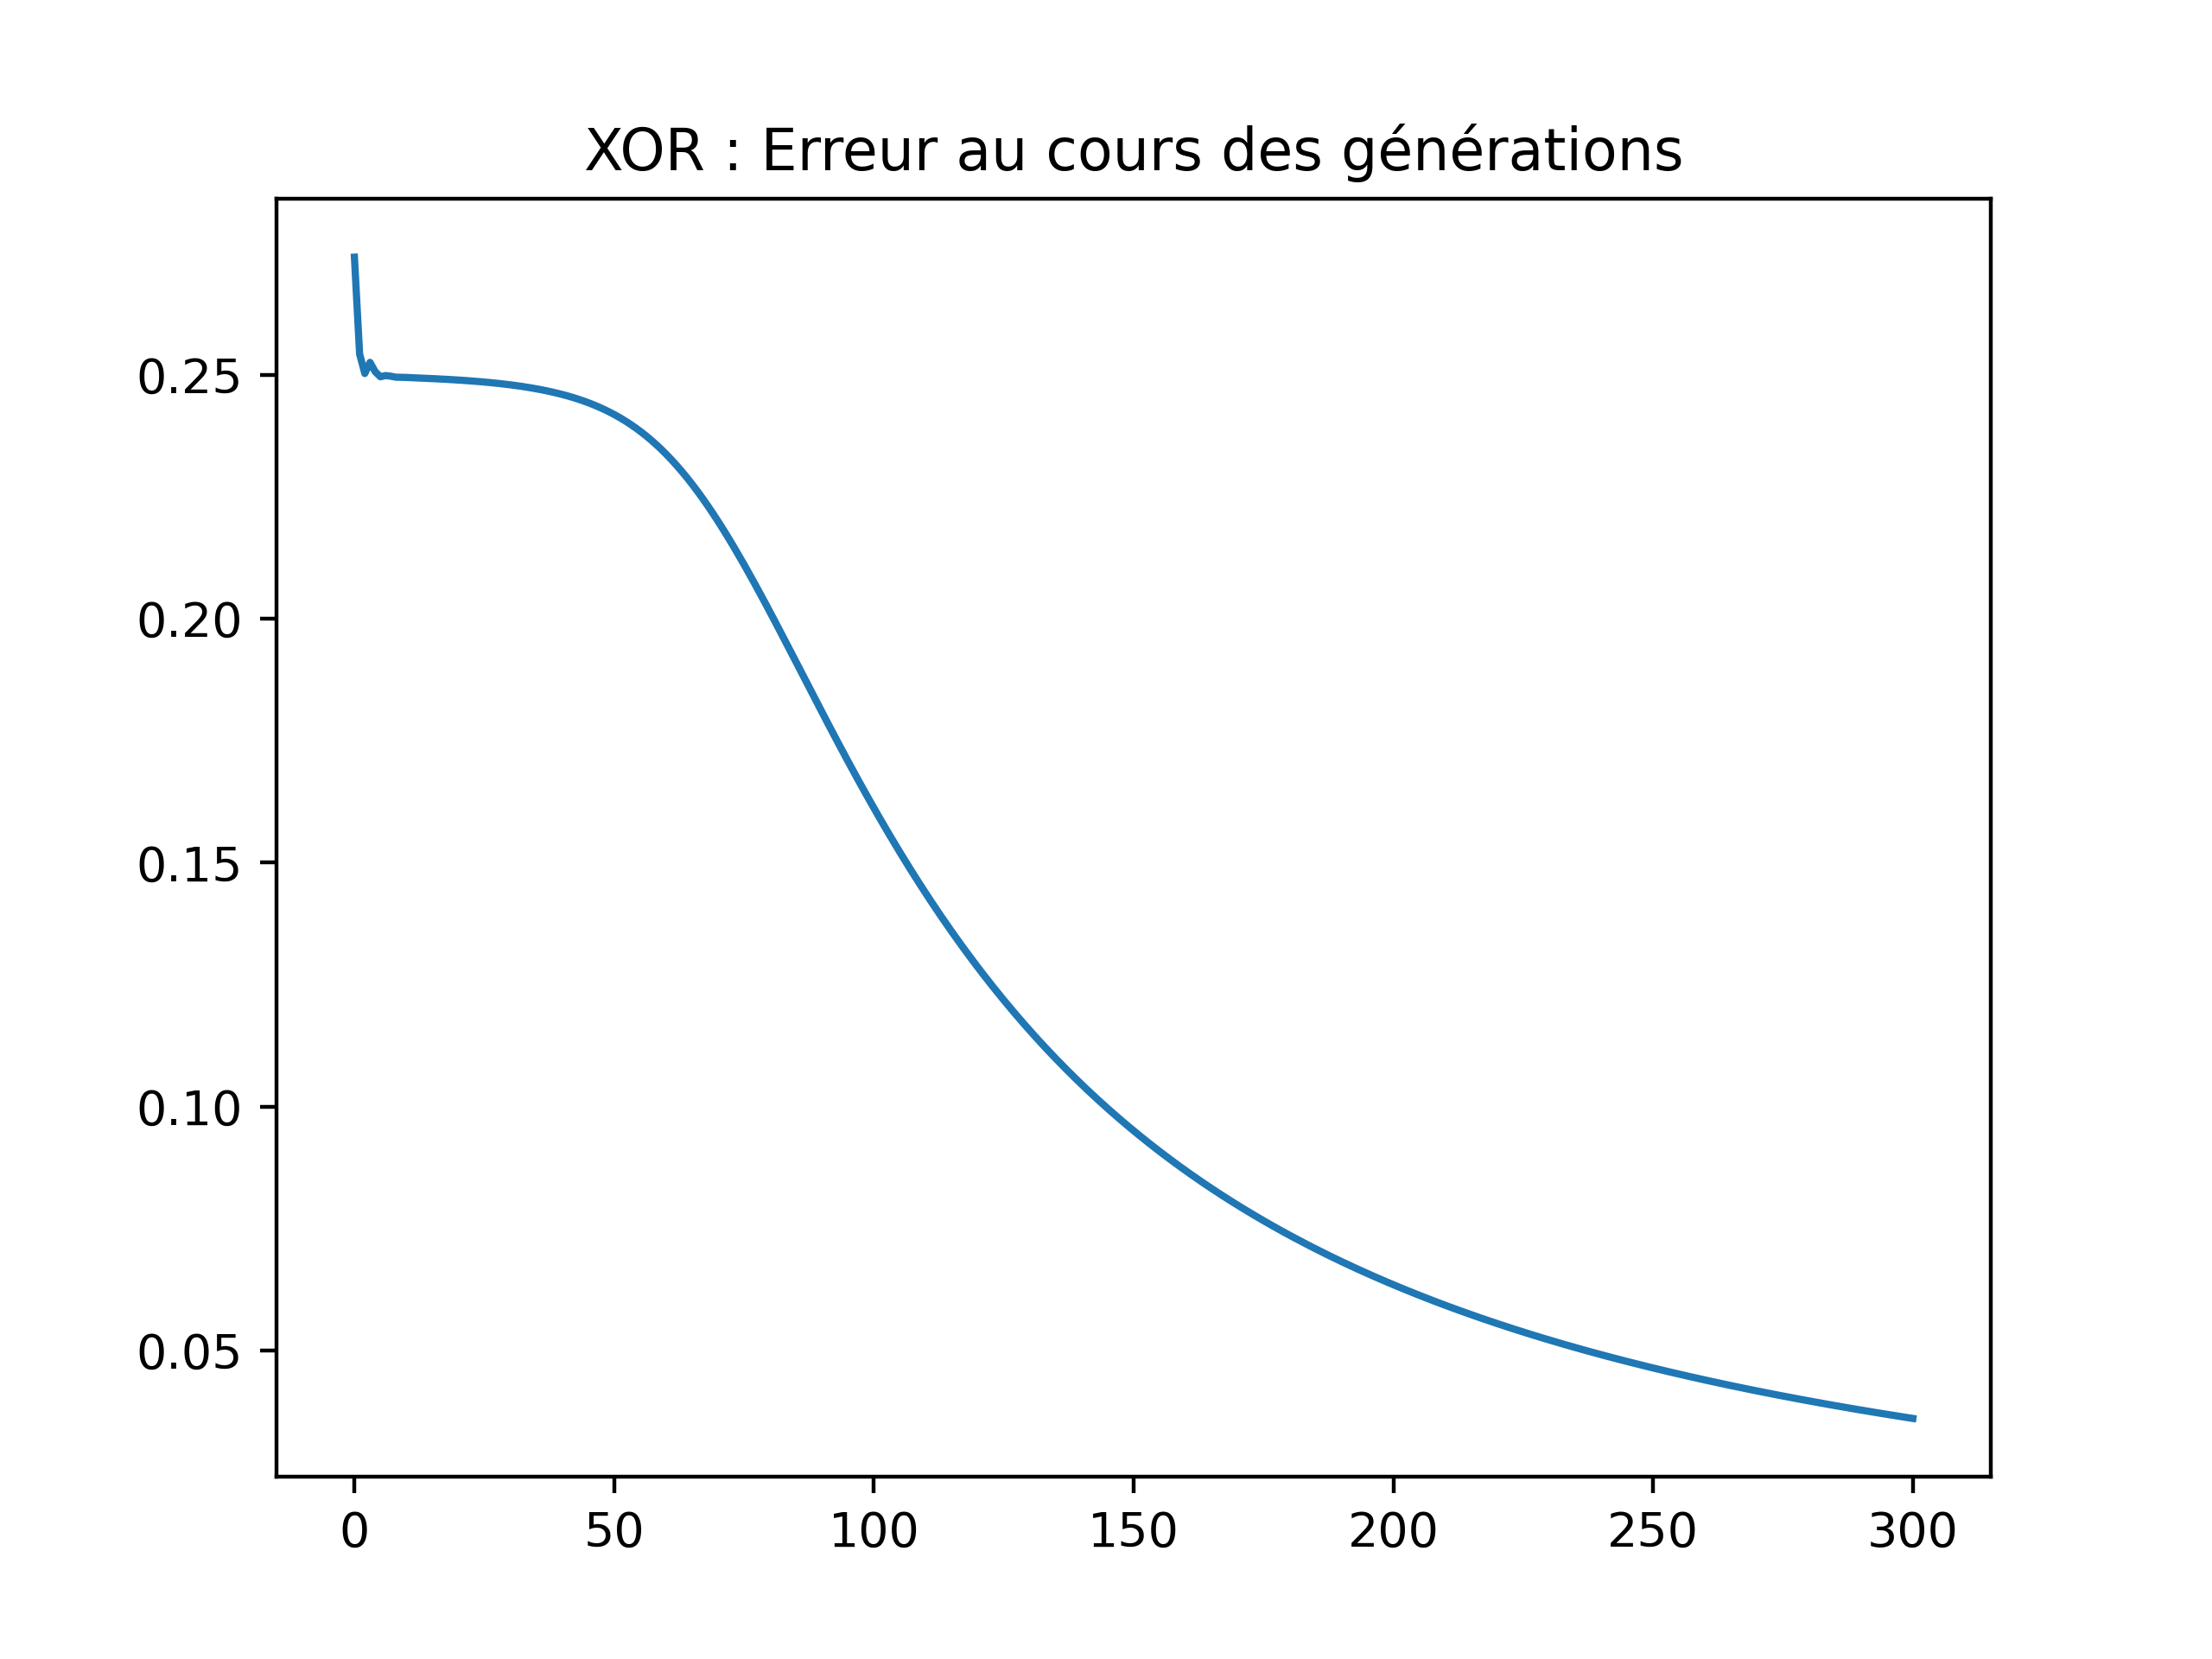
\includegraphics[width=270px]{4-XOR.png}
		\caption{Erreur sur la reproduction du XOR au cours de l'apprentissage}
	\end{figure}
\end{frame}


\begin{frame}{IV - Mes résultat}
	\begin{block}{Données}
		• 4 données \\
		• 300 générations
	\end{block}
	\begin{align*}
		Entr\acute{e} e\, :
		\begin{pmatrix}
			0 & 0 \\
			0 & 1 \\
			1 & 0 \\
			1 & 1
		\end{pmatrix}
		 & \to
		\mathlarger{\mathlarger{\sigma_{couche1}}}
		\left( \centerdot \times
		\begin{pmatrix}
				0.85 & 5.42 \\
				0.85 & 5.40 
			\end{pmatrix}
		\right) \\
		 & \to
		\mathlarger{\mathlarger{\sigma_{couche2}}}
		\left( \centerdot \times
		\begin{pmatrix}
				-18.39 \\
				14.42  
			\end{pmatrix}
		\right) \\
		 & \to
		Sortie\, :
		\begin{pmatrix}
			0.12 \\
			0.81 \\
			0.81 \\
			0.24
		\end{pmatrix}
		Sortie_{attendue}\, :
		\begin{pmatrix}
			0 \\
			1 \\
			1 \\
			0
		\end{pmatrix}
	\end{align*}
\end{frame}